\epigraph{The bad news is time flies. The good news is you're the pilot}
{\textit{Michael Altshuler}}

% There is more to life than just maths basically

% Take up other things - exericse - join socieits - univeristy has so many things to offer - learn how to cook - spend time with friends 

% Continue hobbies 

% How to deal with things overhwelmign and burn out 


\section{Structuring Time}

There is a funny shift that happens in the first few weeks of university. No-one tells you what to do between lectures. 

You might have three lectures in the morning and then nothing scheduled until the following afternoon. That looks like a lot of free time but in reality, it's hours of unstructured time. And unstructured time has a habit of disappearing. 

Time management in a Maths degree isn’t about cramming more hours in, but about avoiding last-minute panic. Maths needs uninterrupted thought. One hour of undistracted thinking is worth more than three hours of broken attention. If you have a two hour gap between lectures, don't assume it's automatically productive time. Decide in advance what you're going to go. Sometimes you might be tired and use that to relax and read a novel or a hit the gym, or maybe you didn't quite understand the last 10 mins of the previous lecture and want to review the notes. It doesn't matter what you do, as long as it's intentional. 

\section{Overworking vs Avoidance}

It’s easy to confuse burnout with avoidance. If you are avoiding starting because the work feels uncomfortable, that’s one thing. Usually once you begin, the momentum builds. However, if you're staring at the page feeling exhausted and unable to process even simple steps, that’s something else. 

Being honest about which one you are experiencing is important. There is no pride in pushing through exhaustion just to prove you can, and equally, there is no growth in endlessly procrastinating out of fear.

If you find yourself consistently overwhelmed, talk to someone. That could be your personal tutor, the \textbf{\href{https://www.southampton.ac.uk/studentservices/support-wellbeing.page}{Student Hub wellbeing team}}, the \textbf{\href{https://www.susu.org/support/university-support.html}{SUSU advice centre}}, or even your friends. University has systems in place because they know how common it is for students to struggle with these things.  

\section{Life Outside the Degree} 

It can be quite easy for your degree to consume everything. And sometimes that feels good, but remember that university is not just a degree factory. 

There are lots of \textbf{\href{https://www.susu.org/activities/}{clubs and societies}}, sports, random Wednesday evenings that end up in unexpectedly good memories. Making time and space for those things is part of the experience, not a distraction. 

I have always found that I think more clearly after stepping away from a problem having spent a considerable amount of time on it. Some of the best insights into problems and questions arrived while I was engaged in something else entirely like cooking or rowing. 

There will be weeks where the workload increases and the social things need to take a slight step back, and there will also be weeks where you might say yes to more events outside of academics. Whatever it might be, balance is not something you're expected to achieve once and then maintain perfectly, it requires constant adjustment. 

If you’re always exhausted, something needs to change. If you’re always disengaged, something also needs to change. Doing a maths degree can feel intense at times as it demands genuine critical thinking. But it still is a degree, not your entire identity. So work hard, and also remember to close the notebook sometimes and have fun. 




\begin{figure}[H]
    \centering
    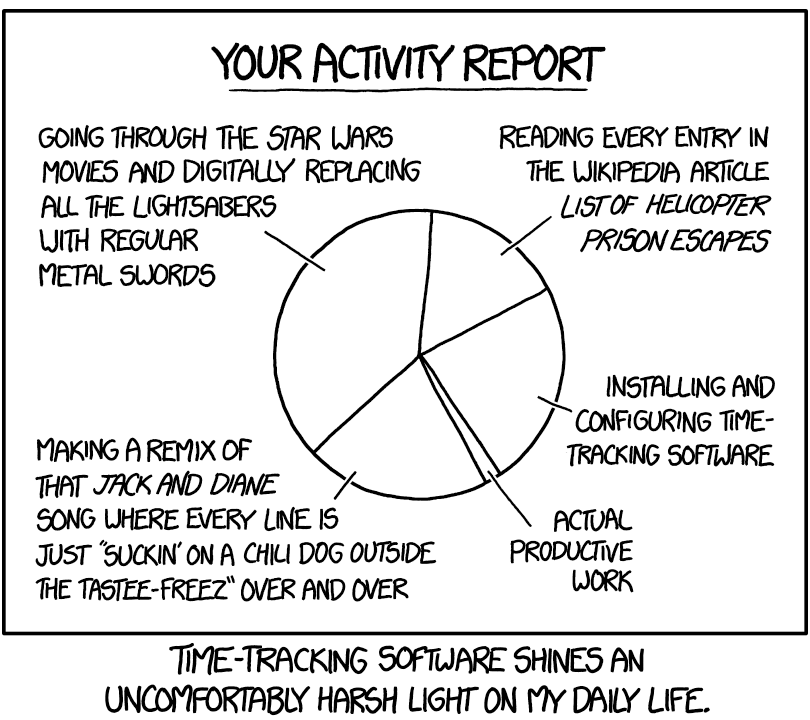
\includegraphics[width=0.5\linewidth]{xkcd/timeTracking.png}
    \caption{\textbf{\href{https://xkcd.com/1690/}{Time-Tracking Software}}}
\end{figure}

\begin{figure}[H]
    \centering
    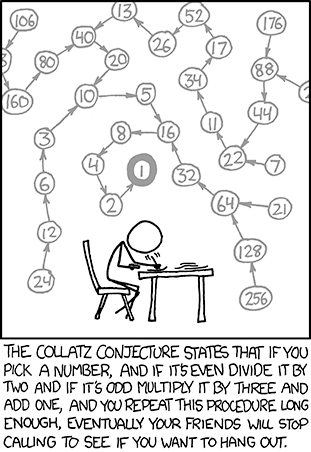
\includegraphics[width=0.4\linewidth]{xkcd/collatzConjecture.png}
    \caption{\textbf{\href{https://xkcd.com/710/}{Collatz Conjecture}}}
\end{figure}

